\section{Soluzioni}

\subsection{Soluzioni di esercizi nella sezione ``\textbf{\nameref{subsec:s_polynomials}}".}

Soluzione dell'esercizio \ref{exp_1} a pagina \pageref{exp_1}\label{poli_1}


\begin{enumerate}
\item List all possible rational zeros of P.

I possibili zeri si trovano usando il \emph{Rational Zero Theorem} :

\begin{enumerate}
\item $p=\pm 1, \pm 3$
\item $q=\pm 1, \pm 2$
\item i possibili valori di $\pm \frac{p}{q}$ sono $\pm 1, \pm \frac{1}{2}, \pm 3, \pm \frac{3}{2}$
\end{enumerate}

\item Find all real zeros of P,

\begin{enumerate}
\item Sostituisco i vari valori di $\pm \frac{p}{q}$:
\setcounter{equation}{0}

\begin{itemize}

\item Provo con $1$:

\begin{equation*}
P(1)=2-5-4+3=-4
\end{equation*}

\item Provo con $-1$:

\begin{equation*}
P(-1)=-2-5+4+3=0 \Leftarrow \textrm{ trovato il primo}
\end{equation*}

\item Provo con $\frac{1}{2}$:

\begin{equation*}
\begin{split}
P\left(\frac{1}{2}\right)&=2\left(\frac{1}{2}\right)^3-5\left(\frac{1}{2}\right)^2-4\left(\frac{1}{2}\right)+3= \\
\\
\frac{2}{8}-\frac{5}{4}-\frac{4}{2}+3&=\frac{2-10-16+24}{8}=0 \Leftarrow \textrm{ trovato il secondo}
\end{split}
\end{equation*}

\item Provo con $-\frac{1}{2}$:

\begin{equation*}
\begin{split}
P\left(-\frac{1}{2}\right)=2\left(-\frac{1}{2}\right)^3&-5\left(-\frac{1}{2}\right)^2-4\left(-\frac{1}{2}\right)+3=\\
\\
-\frac{2}{8}-\frac{5}{4}+\frac{4}{2}+3&=\frac{-2-10+16+24}{8}=\\
\\
\frac{28}{8}&=3.5
\end{split}
\end{equation*}

\item Provo con $3$:

\begin{equation}
\begin{split}
P(3)=2*27-5*9-4*3+3=\\
\\
54-45-12+3=0 \Leftarrow \textrm{ trovato il terzo}
\end{split}
\end{equation}

\end{itemize}



\item Sketch the graph of P.

So che il grafico passa per i punti: $(0,-1)$, $(0, \frac{1}{2})$ e $(0, 3)$.

Calcolo $P(0)=3$ e segno anche quello.

\begin{figure}[H]
\centering
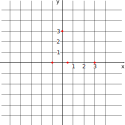
\includegraphics[width=0.5\textwidth]{function.1.pdf}
\end{figure}

Sapendo più o meno la forma delle funzioni di terzo grado posso tracciare questa curva:

\begin{figure}[H]
\centering
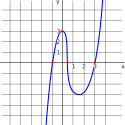
\includegraphics[width=0.5\textwidth]{function.2.pdf}
\end{figure}




\end{enumerate}

Ho trovato tre zeri: $-1$, $\frac{1}{2}$ e $3$.

Non occorre provare gli altri perché una equazione di terzo grado ha al massimo tre zeri.



\item

\end{enumerate}

\subsection{Soluzioni di esercizi nella sezione ``\textbf{\nameref{subsec:val_num}}".}

Soluzione dell'esercizio \ref{exn_1} a pagina \pageref{exn_1}\label{soln_1}
\begin{equation*}
2\log_{12}3+4\log_{12}2=\ldots
\end{equation*}

\begin{equation*}
=\log_{12}3^2+\log_{12}2^4=\log_{12}9+\log_{12}16
\end{equation*}

\begin{equation*}
=\log_{12}144=\log_{12}12^2=2\log_{12}12=2\cdot 1=2
\end{equation*}

\vspace{1cm}
\hrule
\vspace{1cm}

\subsection{Soluzioni di esercizi nella sezione ``\textbf{\nameref{subsec:equazioni}}".}

Soluzione dell' \ref{ex_1} a pagina \pageref{ex_1}\label{sol_1}

\begin{equation*}
\log_2\left(\frac{5}{4}x-1\right)=-2
\end{equation*}

Le equazioni con i logaritmi si risolvono quando tutti i termini sono dei logaritmi.

Quindi bisogna trovare il modo di trasformare tutto ciò che non lo è in un logaritmo.

In questo caso bisogna trovare un valore $a$ tale che 

\begin{equation*}
\log_2(a)=-2
\end{equation*}

cioè 

\begin{equation*}
\begin{split}
2^{-2}&=a \\
\\
\Rightarrow a&=\frac{1}{2^2} \\
\\
\Rightarrow a&=\frac{1}{4} \\
\end{split}
\end{equation*}

A questo punto il problema diventa

\begin{equation*}
\begin{split}
\log_2\left(\frac{5}{4}x-1\right)&=log_2\left(\frac{1}{4}\right) \\
\\
\frac{5}{4}x-1&=\frac{1}{4} \\
\\
\frac{5}{4}x&=\frac{5}{4} \\
\\
x&=1
\end{split}
\end{equation*}

\vspace{1cm}
\hrule
\vspace{1cm}

Soluzione dell'\ref{ex_2} a pagina \pageref{ex_2}\label{sol_2}

\begin{equation*}
\log_22\frac{2x}{x+3}=-1
\end{equation*}



Come nel caso precedente, bisogna trasformare tutti i termini in logaritmi.


Primo passo: trovare $a$ tale che:

\begin{equation*}
\begin{split}
\log_2a=-1\\
\\
2^{-1}=a\\
\\
a=\frac{1}{2}
\end{split}
\end{equation*}

Ora possiamo continuare così:

\begin{equation*}
\begin{split}
\log_2\frac{2x}{x+3}&=log_2\frac{1}{2} \\
\\
\frac{2x}{x+3}&=\frac{1}{2} \\
\\
\frac{4x}{2\cdot(x+3)}&=\frac{x+3}{2\cdot(x+3)} \\
\\
4x&=x+3 \\
\\
x&=1
\end{split}
\end{equation*}


\vspace{1cm}
\hrule
\vspace{1cm}
Soluzione dell'\ref{ex_3} a pagina \pageref{ex_3}\label{sol_3}

\begin{equation*}
\log_2(w^2+4w+3)=4+\log_2(w^2+w)
\end{equation*}

\begin{equation*}
\Rightarrow\log_2(w^2+4w+3)-\log_2(w^2+w)=4
\end{equation*}

\begin{equation*}
\Rightarrow
\log_2\left(\frac{
w^2+4w+3
}{
w^2+w
}\right) = 4\log_22
\end{equation*}

\begin{equation*}
\log_2\left(\frac{
(w+1)(w+3)
}{
w(w+1)
}\right) = 4\log_22 \textrm{ ($w\neq -1$)}
\end{equation*}

\begin{equation*}
\log_2\left(\frac{w+3}{w}\right) = \log_216
\end{equation*}

\begin{equation*}
\frac{w+3}{w}=16
\end{equation*}

\begin{equation*}
w+3=16w
\end{equation*}

\begin{equation*}
w=\frac{1}{5}
\end{equation*}

\vspace{1cm}
\hrule
\vspace{1cm}


\subsection{Soluzioni di esercizi nella sezione ``\textbf{\nameref{subsec:mult_choice}}".}

Quesiti a pagina \pageref{ex_mc}
\label{sol_mc}

\begin{enumerate}
\item A, B, D
\item A
\item C
\end{enumerate}

\vspace{1cm}
\hrule
\vspace{1cm}

Soluzione dell'esercizio \ref{ex_4_5} a pagina \pageref{ex_4_5}\label{sol_4_5}

\begin{equation*} % completare
ln(lg 10)+ \sqrt{(\pi -4)^2}=\ldots?
\end{equation*}


\begin{equation*}
ln(lg 10)+ \sqrt{(\pi -4)^2}=\ldots
\end{equation*}

\begin{equation*}
\ln(log_{10} 10) +(4-\pi)=
\end{equation*}

\begin{equation*}
\ln1+4-\pi=
\end{equation*}

\begin{equation*}
4-\pi
\end{equation*}





\vspace{1cm}
\hrule
\vspace{1cm}






Soluzione dell'esercizio \ref{ex_5} a pagina \pageref{ex_5}\label{sol_5}

Data la seguente funzione:

\begin{equation*}
f(3x)=\log_2{\sqrt{\frac{9x+1}{2}}}
\end{equation*}

Quanto vale $f(1)$?


Questa è una funzione composta:

\begin{equation*}
f(g(x)) \textrm{ con } g(x)=3x
\end{equation*}

O se preferiamo $y=3x$

Quindi 

\begin{equation*}
x=\frac{y}{3}
\end{equation*}

\begin{equation*}
f(y)=\log_2{\sqrt{\frac{9\frac{y}{3}+1}{2}}}
\end{equation*}

Ora basta sostituire $y$ con $1$

\begin{equation*}
f(1)=\log_2{\sqrt{\frac{9\frac{1}{3}+1}{2}}}
\end{equation*}



\vspace{1cm}
\hrule
\vspace{1cm}
Soluzione dell'esercizio \ref{ex_6} a pagina \pageref{ex_6}\label{sol_6}

Trovare il valore di $\frac{x^2}{y}$ sapendo che 

\begin{equation*}
\begin{split}
\log_{\frac{1}{2}}x=m \\
\\
\log_{\frac{1}{4}}y=m+2
\end{split}
\end{equation*}

\vspace{1cm}
\hrule
\vspace{1cm}

Soluzione

Uso la formula del il cambiamento di base

\begin{equation*}
\log_{\frac{1}{4}}y=\frac{
\log_{\frac{1}{2}}y
}{
\log_{\frac{1}{2}}\frac{1}{4}
}=m+2
\end{equation*}

ma $\log_{\frac{1}{2}}\frac{1}{4}$ fa 2, quindi

\begin{equation*}
\log_\frac{1}{2}y=2(m+2)
\end{equation*}

Ora posso cambiare i logaritmi in potenze:

\begin{equation*}
\begin{split}
\frac{1}{2}^m=x \\
\\
\frac{1}{2}^{2m+2}=y
\end{split}
\end{equation*}

\begin{equation*}
\frac{x^2}{y}=
\frac{
\left( \left( \frac{1}{2} \right)^m \right)^2
}{
\left( \frac{1}{2} \right) ^{(2m+2)}
}
\end{equation*}

\begin{equation*}
\frac{
\left( \frac{1}{2} \right)^{2m}
}{
\left( \frac{1}{2} \right) ^{2m} \cdot
\frac{1}{2}^2
}=4
\end{equation*}

\vspace{1cm}
\hrule
\vspace{1cm}



Soluzione dell'esercizio \ref{ex_7} a pagina \pageref{ex_7}\label{sol_7}

\begin{equation*}
\log_3(x+1)=3-log_3(x+7)
\end{equation*}

Soluzione

\begin{equation*}
\log_3(x+1)+log_3(x+7)=3
\end{equation*}

\begin{equation*}
\log_3[(x+1) \cdot (x+7)]=3
\end{equation*}

\begin{equation*}
3^3=(x+1) \cdot (x+7)
\end{equation*}



\vspace{1cm}
\hrule
\vspace{1cm}


\begin{minipage}{\textwidth}
Soluzione dell'esercizio \ref{ex_8} a pagina \pageref{ex_8}\label{sol_8}

\begin{equation*}
\log(x^2)=(log(x))^2 
\end{equation*}

Soluzione

\begin{equation*}
2\cdot \log(x)=(log(x))^2 
\end{equation*}

\begin{equation*}
\log(x)\cdot (log(x)-2)-0
\end{equation*}

Ci sono due risultati:

\begin{equation*}
\log(x)=0\textrm{ ma anche }log(x)=2
\end{equation*}

In forma di potenza abbiamo

\begin{equation*}
10^0=x \textrm{ , } 10^2=x
\end{equation*}

Le soluzioni sono quindi

\begin{equation*}
x_1=1 \textrm{ , } x_2=100
\end{equation*}

\end{minipage}



\vspace{1cm}
\hrule
\vspace{1cm}

Soluzione dell'esercizio \ref{ex_9} a pagina \pageref{ex_9}\label{sol_9}

\begin{equation*}
\log(x-1)-log(x+1)=log(x-3)-log(x-2)
\end{equation*}

\begin{equation*}
\log\left(\frac{x-1}{x+1}\right)=log\left(\frac{x-3}{x-2}\right)
\end{equation*}

\begin{equation*}
\frac{x-1}{x+1}=\frac{x-3}{x-2}
\end{equation*}


\begin{equation*}
x^2-3x+2=x^2-2x-3
\end{equation*}

\begin{equation*}
x=5
\end{equation*}



\vspace{1cm}
\hrule
\vspace{1cm}

Soluzione dell'esercizio \ref{ex_10} a pagina \pageref{ex_10}\label{sol_10}


Trovare $x$ per 


% da https://assets.cambridge.org/97811076/53153/excerpt/9781107653153_excerpt.pdf
\begin{equation*}
4\cdot 5^{x+1} = 3^x
\end{equation*}

Siccome l'incognita è un esponente di una potenza, per tirarla giù usiamo i logaritmi.

\begin{equation*}
\log(4\cdot 5^{x+1}) = log(3^x)
\end{equation*}

\begin{equation*}
\log 4+log(5^{x+1}) = log(3^x)
\end{equation*}

\begin{equation*}
\log 4 +(x+1)\log5 = x\cdot \log3
\end{equation*}

\begin{equation*}
\log4 +x\cdot \log5+\log5 = x\cdot \log3
\end{equation*}

\begin{equation*}
x(\log3-\log5)=\log4+\log5
\end{equation*}

\begin{equation*}
x=\frac{
\log4+\log5
}{
\log3-\log5
}
\end{equation*}



\vspace{1cm}
\hrule
\vspace{1cm}

Soluzione dell'esercizio \ref{ex_11} a pagina \pageref{ex_11}\label{sol_11}

\begin{equation*}
3^{2x+1}-11\cdot 3^x=4
\end{equation*}


Ci sono $3^{2x+1}$ e $3^x$, sono tutti parenti di $3^x$, trasformiamo tutto in termini di $3^x$

\begin{equation*}
3\cdot 3^{2x}-11\cdot 3^x=4
\end{equation*}

\begin{equation*}
3\cdot {\left(3^x\right)}^2-11\cdot 3^x=4
\end{equation*}

Ora diciamo che $y=3^x$, in modo che diventi una normale quadratica:

\begin{equation*}
3y^2-11y-4=0
\end{equation*}

\begin{equation*}
(3y+1)(x-4)=0
\end{equation*}

\begin{equation*}
y_1=-\frac{1}{3}\textrm{\hspace{1cm}}y_2=4
\end{equation*}

Questo significa che $3^x$ può essere $-\frac{1}{3}$ oppure $4$.

$3^x=-\frac{1}{3}$ è impossibile perché $3^x$ è sempre positivo, quindi

\begin{equation*}
3^x=4
\end{equation*}

\begin{equation*}
\log3^x=\log4
\end{equation*}

\begin{equation*}
x\log3=\log4
\end{equation*}

\begin{equation*}
x=\frac{\log4}{\log3}
\end{equation*}

\vspace{1cm}
\hrule
\vspace{1cm}

Soluzione dell'esercizio \ref{ex_12} a pagina \pageref{ex_12}\label{sol_12}

Date le relazioni:

\begin{itemize}
\item $x = \log a$
\item $y = \log b$
\item $z = \log c$
\end{itemize}

Scrivere $2x+y-\frac{1}{2}z+2$ come un singolo logaritmo $\log(W)$.

Soluzione:

Il punto di partenza è questo:

\begin{equation*}
2\log a+\log b-\frac{1}{2}\log c+2
\end{equation*}

Per usare le regole dei logaritmi non ci devono essere coefficienti, quindi li portiamo dentro:

\begin{equation*}
\log a^2+\log b-\log c^{\frac{1}{2}}+2
\end{equation*}

Adesso possiamo scrivere

\begin{equation*}
\log a^2b-\log  c^{\frac{1}{2}}+2
\end{equation*}

\begin{equation*}
=\log\left(
\frac{
a^2b
}{
\sqrt{c}
}
\right)+2
\end{equation*}

\begin{equation*}
=\log\left(
\frac{
a^2b
}{
\sqrt{c}
}
\right)+\log100
\end{equation*}

\begin{equation*}
=\log\left(
\frac{
100\cdot a^2b
}{
\sqrt{c}
}
\right)
\end{equation*}



\vspace{1cm}
\hrule
\vspace{1cm}

Soluzione dell'esercizio \ref{ex_13} a pagina \pageref{ex_13}\label{sol_13}

\begin{equation*}
4\log_4 x=9\log_x 4
\end{equation*}

Per poter fare qualcosa bisogna prima avere i logaritmi nella stessa base.

Usiamo la regola del cambiamento di base:

\begin{equation*}
\log_x 4=\frac{
\log_4 4
}{
\log_4 x
}=\frac{
1
}{
\log_4 x
}
\end{equation*}

Quindi l'equazione data diventa:

\begin{equation*}
4\log_4 x=9 \cdot\frac{
1
}{
\log_4 x
}
\end{equation*}


\begin{equation*}
4(\log_4 x)^2 = 9
\end{equation*}

\begin{equation*}
(\log_4 x)^2 = \frac{9}{4}
\end{equation*}

\begin{equation*}
\sqrt{(\log_4 x)^2} = \sqrt{\frac{9}{4}}
\end{equation*}


\begin{equation*}
\left\{
\begin{array}{ll}
\log_4 x=+\frac{3}{2}\\
\\
\log_4 x=-\frac{3}{2}
\end{array}
\right.
\end{equation*}


\begin{equation*}
\left\{
\begin{array}{ll}
x=4^{\frac{3}{2}}=-8\\
x=4^{-\frac{3}{2}}=\frac{1}{8}
\end{array}
\right.
\end{equation*}


\vspace{1cm}
\hrule
\vspace{1cm}


Soluzione dell'esercizio \ref{exf_1} a pagina \pageref{exf_1}\label{solf_1}

\begin{center}
\fbox{\begin{minipage}{0.9\textwidth}
When a cup of tea is made, its temperature is $85^\circ$C.

After 3 minutes the tea has cooled to $60^\circ$C.

That the temperature $T(^\circ C)$ of the cup of tea decays exponentially according to the function
\begin{equation*}
T = A + Ce^{-0.2t}
\end{equation*}
, where $t$ is the time measured in minutes.

Find:\begin{itemize}
\item the values of $A$ and $C$
\item the time it takes for the tea to cool to $40^\circ$C.
\end{itemize}

\end{minipage}}
\end{center}

\vspace{1cm}

Solution:

\setcounter{equation}{0}
\begin{equation}\label{e1}
\textrm{when }t=0\textrm{ : }85=A+C
\end{equation}

\begin{equation}\label{e2}
\textrm{when }t=3\textrm{ : }60=A+Ce^{-0.6}
\end{equation}

The difference of \ref{e1} - \ref{e2} gives

\begin{equation*}
25=C(1-e^{-0.6})
\end{equation*}

So


\begin{equation*}
C=\frac{25}{1-e^{-0.6}}=55.4
\end{equation*}

From equation \ref{e1}:

\begin{equation*}
A=85-C=85-55.4=29.6
\end{equation*}

\begin{minipage}{\textwidth}
Now for finding the time, when $T=40$:


\begin{equation*}
29.6+55.4e^{-0.2t}=40
\end{equation*}


\begin{equation*}
e^{-0.2t}=\frac{40-29.6}{55.4}
\end{equation*}

\begin{equation*}
ln\left(e^{-0.2t}\right)=
ln\left(
\frac{40-29.6}{55.4}
\right)
\end{equation*}

\begin{equation*}
-0.2t=ln\left(
\frac{40-29.6}{55.4}
\right)
\end{equation*}

$t=8.36$ minutes.
\end{minipage}



\vspace{1cm}
\hrule
\vspace{1cm}


Soluzione dell'esercizio \ref{exf_2} a pagina \pageref{exf_2}\label{solf_2}

Math Olympiad question!

\begin{equation*}
25^x-15^x=9^x
\end{equation*}

Soluzione:

\begin{equation*}
\frac{25^x}{9^x}-
\frac{15^x}{9^x}=
\frac{9^x}{9^x}
\end{equation*}

\begin{equation*}
\left(
\frac{25}{9}
\right)^x
-
\left(
\frac{15}{9}
\right)^x
=1
\end{equation*}

\begin{equation*}
\left( \frac{ 5^2}{ 3^2} \right)^x
-
\left(
\frac{5\cdot 3}
{3\cdot 3} 
\right)^x=1
\end{equation*}

\begin{equation*}
\left[ \left( \frac{5}{3} \right)^2 \right]^x
-
\left(
\frac{5}
{3} 
\right)^x=1
\end{equation*}

\begin{equation*}
\left[ \left( \frac{5}{3} \right)^x \right]^2
-
\left(
\frac{5}
{3} 
\right)^x=1
\end{equation*}


\begin{equation*}
\textrm{Ora poniamo } t=\left( \frac{5}{3} \right)^x
\end{equation*}


\begin{equation*}
\textrm{Abbiamo } t^2-t-1=0
\end{equation*}

\begin{equation*}
t=\frac{ 1\pm \sqrt{5} }{2 }
\end{equation*}

\begin{equation*}
\left( \frac{5}{3} \right)^x=\frac{ 1+ \sqrt{5} }{2 }
\end{equation*}

\begin{equation*}
\log\left( \frac{5}{3} \right)^x=\log\left(\frac{ 1+ \sqrt{5} }{2 }\right)
\end{equation*}

\begin{equation*}
x\cdot \log\left( \frac{5}{3} \right)=\log\left(\frac{ 1+ \sqrt{5} }{2 }\right)
\end{equation*}

\begin{equation*}
x(\log5-log3)=\log(1+\sqrt 5)-\log2
\end{equation*}

\begin{equation*}
x=\frac
{\log(1+\sqrt 5)-\log2}
{\log5-\log3}
\end{equation*}


\vspace{1cm}
\hrule
\vspace{1cm}



Soluzione dell'esercizio \ref{exf_3} a pagina \pageref{exf_3}\label{solf_3}

\begin{equation*}
100^{\left(\frac{1}{2}\lg9-lg2\right)}-\log_98\cdot\log_4\sqrt[3]{3}
\end{equation*}

100 è $10^2$; poi converto i $\log_9$ e $\log_4$ in $\lg$; poi $\sqrt[3]{3}=3^{\frac{1}{3}}$

\begin{equation*}
10^{2^{\left(\frac{1}{2}\lg9-\lg2\right)}}-\frac{\lg8}{\lg9}\cdot\frac{1}{3}\log_43
\end{equation*}

\begin{equation*}
10^{\left(\lg9-\lg4\right)}-\frac{3\lg2}{2\lg3}\cdot\frac{\lg3}{3\lg4}
\end{equation*}

\begin{equation*}
\frac{10^{\lg9}}{10^{\lg4}}-\frac{3\lg2}{2\lg3}\cdot\frac{\lg3}{6\lg2}
\end{equation*}

Attenzione: $a^{\log_ab}=b$ quindi $10^{\lg9}=9$ e $10^{\lg4=4}$

\begin{equation*}
\frac{9}{4}-\frac{3}{12}=2
\end{equation*}



\vspace{1cm}
\hrule
\vspace{1cm}

\subsection{Soluzioni di esercizi nella sezione ``\textbf{\nameref{subsec:ss_trigo}}".}



Soluzione dell'esercizio \ref{etri_01} a pagina \pageref{etri_01}\label{stri_01}

BC è facile perché ABC è un triangolo retto, si può usare il teorema di Pitagora.


\begin{equation*}
\sqrt{{AB}^2-{AC}^2}=
\sqrt{{220}^2-{180}^2}=
\end{equation*}

\begin{equation*}
\sqrt{48400 - 32400}=\sqrt{16000}=126.49
\end{equation*}

Per la seconda parte si usa il teorema di Carnot (a pagina \pageref{subs_carnot})

\begin{equation*}
DC^2=AD^2+AC^2-2\cdot AD\cdot AC\cdot \cos(33^\circ)=
\end{equation*}

\begin{equation*}
170^2+180^2-2\cdot 170\cdot 180 * 0.838=
\end{equation*}

\begin{equation*}
28900+32400-51285.6=10014.4
\end{equation*}

DC=$\sqrt{10014.4}$=$100.071$

\vspace{1cm}
\hrule
\vspace{1cm}

Soluzione dell'esercizio \ref{etri_02} a pagina \pageref{etri_02}\label{stri_02}

Il problema si riduce a trovare il cateto maggiore di un triangolo di cui si conosce il cateto minore e due angoli.

\begin{figure}[H]
\centering

\includegraphics[width=0.3\textwidth]{trigo_06.pdf}
\end{figure}

L'incognita è $b$.

Gli elementi conosciuti sono:
\begin{itemize}
\item[$\beta$] = $82^{\circ}$
\item[$\alpha$] = $90^{\circ}$
\item[$c$] = $50$
\end{itemize}

L'angolo $\gamma$ è pari a $180-90-82=8^{\circ}$

Grazie al Teorema di Eulero (pagina \pageref{subs_euler}) sappiamo che 


\begin{equation*}
\frac{a}{\sin (\alpha)} = \frac{b}{\sin (\beta)} = \frac{c}{\sin (\gamma)}
\end{equation*}

quindi

\begin{equation*}
\frac{b}{\sin (82)} = \frac{50}{\sin (8)}
\end{equation*}

\begin{equation*}
b=\frac{50\cdot 0.990}{0.139}=356.115\textrm{ metri}
\end{equation*}

\vspace{1cm}
\hrule
\vspace{1cm}

\begin{minipage}{\textwidth}
Soluzione dell'esercizio \ref{etri_03} a pagina \pageref{etri_03}\label{stri_03}


\begin{equation*}
\frac{
\cos(x)
}{
\tan(x)\cdot\left(1-\sin(x)\right)
} = 1+\frac{1}{\sin(x)}
\end{equation*}


Per prima cosa moltiplico tutto per $\tan(x)$:

\begin{equation*}
\Rightarrow\frac{
\cos(x)
}{
\left(1-\sin(x)\right)
} = \tan(x)+\frac{\tan(x)}{\sin(x)}
\end{equation*}

Poi sostitsco $\tan(x)=\frac{\sin(x)}{\cos(x)}$:


\begin{equation*}
\Rightarrow\frac{
\cos(x)
}{
\left(1-\sin(x)\right)
} = \frac{\sin(x)}{\cos(x)}+\frac{1}{\cos(x)}
\end{equation*}

Porto $\frac{\sin(x)}{\cos(x)}$ a sinistra:

\begin{equation*}
\Rightarrow\frac{
\cos(x)
}{
\left(1-\sin(x)\right)
} 
-
\frac{\sin(x)}{\cos(x)}
= \frac{1}{\cos(x)}
\end{equation*}

Moltiplico $\frac{
\cos(x)
}{
\left(1-\sin(x)\right)
}$ per $\frac{\cos(x)}{\cos(x)}$ (che sarebbe $1$):

\begin{equation*}
\Rightarrow
\frac{\cos(x)}{\cos(x)}
\cdot
\frac{
\cos(x)
}{
\left(1-\sin(x)\right)
} 
-
\frac{\sin(x)}{\cos(x)}
= \frac{1}{\cos(x)}
\end{equation*}

\begin{equation*}
\Rightarrow
\frac{\cos^2(x)}{\cos(x)
\cdot
\left(1-\sin(x)\right)
} 
-
\frac{\sin(x)}{\cos(x)}
= \frac{1}{\cos(x)}
\end{equation*}

Moltiplico $\frac{\sin(x)}{\cos(x)}$ per $\frac{1-\sin(x)}{1-\sin(x)}$:

\begin{equation*}
\Rightarrow
\frac{\cos^2(x)}{\cos(x)
\cdot
\left(1-\sin(x)\right)
} 
-
\frac{\sin(x)}{\cos(x)}
\cdot
\frac{1-\sin(x)}{1-\sin(x)}
= \frac{1}{\cos(x)}
\end{equation*}

In questo modo i denominatori sono uguali quindi posso raccogliere:

\begin{equation*}
\Rightarrow
\frac{
\cos^2(x)-\sin(x)+\sin^2(x)}
{
\cos(x)\cdot
\left(1-\sin(x)\right)
} 
= \frac{1}{\cos(x)}
\end{equation*}

So che $\cos^2(x)+\sin^2(x)=1$:

\begin{equation*}
\Rightarrow
\frac{
1-\sin(x)
}{
\cos(x)\cdot
\left(1-\sin(x)\right)
} 
= \frac{1}{\cos(x)}
\end{equation*}

Semplifico togliendo $1-\sin(x)$:


\begin{equation*}
\Rightarrow
\frac{
1
}{
\cos(x)
} 
= \frac{1}{\cos(x)}
\end{equation*}

\end{minipage}
Soluzione dell'esercizio \ref{etri_04} a pagina \pageref{etri_04}\label{stri_04}

\begin{equation*}
\frac{
1+2\sin(x)\cos(x)
}{
\sin(x)+\cos(x)
}
=
\sin(x)+\cos(x)
\end{equation*}


\begin{equation*}
\Rightarrow
\frac{
1+2\sin(x)\cos(x)
}{
\sin(x)+\cos(x)
}
-(\sin(x)+\cos(x))
=
0
\end{equation*}

\begin{equation*}
\Rightarrow
\frac{
1+2\sin(x)\cos(x)
}{
\sin(x)+\cos(x)
}
-\frac{
\sin(x)+\cos(x)
}{
\sin(x)+\cos(x)
}\cdot(\sin(x)+\cos(x))
=
0
\end{equation*}


\begin{equation*}
\Rightarrow
\frac{
1+2\sin(x)\cos(x)
-(
\sin(x)+\cos(x)
)^2
}{
\sin(x)+\cos(x)
}
=
0
\end{equation*}


\begin{equation*}
\Rightarrow
\frac{
1+2\sin(x)\cos(x)
-(
\sin^2(x)+2\sin(x)\cos(x)+\cos^2(x)
)
}{
\sin(x)+\cos(x)
}
=
0
\end{equation*}


\begin{equation*}
\Rightarrow
\frac{
1+2\sin(x)\cos(x)
-\sin^2(x)-2\sin(x)\cos(x)-\cos^2(x)
}{
\sin(x)+\cos(x)
}
=
0
\end{equation*}


\begin{equation*}
\Rightarrow
\frac{
1+2\sin(x)\cos(x)-2\sin(x)\cos(x)-1
}{
\sin(x)+\cos(x)
}
=
0
\end{equation*}


\vspace{1cm}
\hrule
\vspace{1cm}


Soluzione dell'esercizio \ref{analyzem01_l} a pagina \pageref{analyzem01_l}\label{analyzem01_s}

Il raggio $R$ del cerchio dato è uguale a $8$.

La formula per calcolare la lunghezza dell'arco dato il raggio e l'angolo $\theta$ è questa:

\begin{equation*}
S=R\cdot\theta
\end{equation*}

quindi 

\begin{equation*}
20 = 8 \cdot \theta 
\end{equation*}

da cui 
\begin{equation*}
\theta =\frac{20}{8} = 2.5 \textrm{ (in radianti)}
\end{equation*}

Sapendo l'angolo $\theta$ si usano le definizioni di seno e coseno per calcolare le coordinate:

\begin{equation*}
x=R\cdot\cos(\theta) = 8\cdot (2.5) = -6.40
\end{equation*}
\begin{equation*}
y = R\cdot \sin(\theta) = 8 \sin(2.5) = 4.79
\end{equation*}
%We now use the definitions for sine and cosine to find the coordinates x and y of P.
%cos(θ) = x / R     and     sin(θ) = y / R
%cos(θ) = x / R     gives     x = R cos(θ) = 8 cos(2.5) = -6.40
%sin(θ) = y / R     gives     y = R sin(θ) = 8 sin(2.5) = 4.79
%Point P has the coordinates (-6.40 , 4.79).

\subsection{Soluzioni di esercizi nella sezione ``\textbf{\nameref{subsec:additional_log}}".}


Soluzione dell'esercizio \ref{exa_1} a pagina \pageref{exa_1}\label{sola_1}

\begin{equation*}
2\cdot \ln(6x - 2) = 5
\end{equation*}

\begin{equation*}
\ln(6x - 2) = \frac{5}{2}
\end{equation*}

\begin{equation*}
e^{\ln(6x - 2)} = e^{\frac{5}{2}}
\end{equation*}


\begin{equation*}
6x - 2 = e^{\frac{5}{2}}
\end{equation*}

\begin{equation*}
6x = 2+e^{\frac{5}{2}}
\end{equation*}


\begin{equation*}
x = \frac{2+e^{\frac{5}{2}}}{6}
\end{equation*}


\vspace{1cm}
\hrule
\vspace{1cm}

Soluzione dell'esercizio \ref{exa_2} a pagina \pageref{exa_2}\label{sola_2}

\begin{equation*}
e^{4x} - 3e^{2x} + 2 = 0
\end{equation*}


\begin{equation*}
\textrm{Poniamo }u=e^{2x}
\end{equation*}


\begin{equation*}
u^2-3u+2=0
\end{equation*}


\begin{equation*}
(u - 1)(u - 2) =0
\end{equation*}

\begin{equation*}
\left\{
\begin{array}{ll}
u=1 \\
u=2
\end{array}
\right.
\end{equation*}

\begin{equation*}
\left\{
\begin{array}{ll}
e^{2x}=1 \\
e^{2x}=2
\end{array}
\right.
\end{equation*}

\begin{equation*}
\left\{
\begin{array}{ll}
2x=\ln1 \\
2x=\ln2
\end{array}
\right.
\end{equation*}

\begin{equation*}
\left\{
\begin{array}{ll}
x=0 \\
x=\frac{\ln2}{2}
\end{array}
\right.
\end{equation*}



\vspace{1cm}
\hrule
\vspace{1cm}

Soluzione dell'esercizio \ref{exa_3} a pagina \pageref{exa_3}\label{sola_3}


\begin{equation*}
3^xe^{4x-1} = 5
\end{equation*}

\begin{equation*}
\ln ( 3^xe^{4x - 1} ) = \ln 5
\end{equation*}

\begin{equation*}
\ln 3^x + \ln ( e^{4x - 1} ) = \ln 5
\end{equation*}

\begin{equation*}
x\ln 3+4x-1=\ln 5
\end{equation*}

\begin{equation*}
x(\ln3 +4)=\ln 5 +1
\end{equation*}

\begin{equation*}
x=\frac{
1+\ln 5
}{
4+\ln 3
}
\end{equation*}

\vspace{1cm}
\hrule
\vspace{1cm}

\begin{minipage}{\textwidth}
Soluzione dell'esercizio \ref{exa_4} a pagina \pageref{exa_4}\label{sola_4}

La formula data è: 

\begin{equation*}
P = 1000 \cdot 1.0224t
\end{equation*}

Vogliamo $P=2000$, quindi 

\begin{equation*}
2000 = 1000 \cdot 1.022^{4t}
\end{equation*}

\begin{equation*}
2= 1.022^{4t}
\end{equation*}

Applichiamo il logaritmo da entrambe le parti:

\begin{equation*}
4t\cdot \lg 1.022 = \lg 2
\end{equation*}


\begin{equation*}
t=\frac{
\lg 2
}{
4\cdot\lg 1.022
} = 7.96
\end{equation*}

$\approx$ 8 years

\end{minipage}

\vspace{1cm}
\hrule
\vspace{1cm}


\subsection{Soluzioni di esercizi nella sezione ``\textbf{\nameref{subsec:calcolo_combinatorio}}".}

Soluzione dell'esercizio \ref{combl_01} a pagina \pageref{combl_01}\label{combs_01}

Ricordiamoci che 
\begin{equation*}
\binom{n}{k}=\frac{n!}{(n-k)!\cdot k!}
=\frac{
n\cdot(n-1)\times \cdots \times (n-k+1)
}{
k\cdot(k-1)\times \cdots \times 1
}
\end{equation*}

quindi

\begin{equation*}
\binom{n}{8}=\binom{n}{6}
\hspace{1cm}\Rightarrow \hspace{1cm}
\frac{n!}{(n-8)! \cdot 8!} = \frac{n!}{(n-6)! \cdot 6!}
\end{equation*}


\begin{equation*}
\frac{
\cancel{n} \cdot \cancel{(n-1)}\cdot(n-2) \cdots (n-7)\cdot \cancel{(n-8)}!
}
{
\cancel{(n-8)!} \cdot 8 \cdot 7 \cdot \cancel{6!}
} = \frac{
\cancel{n}\cdot\cancel{(n-1)}\cdots(n-5)\cancel{(n-6)!}
}{
\cancel{(n-6)!}\cdot\cancel{6!}
}
\end{equation*}

\begin{equation*}
(n-6)(n-7) = 56
\end{equation*}

$n=14; 14\ge 8 \Rightarrow $OK!

\vspace{1cm}
\hrule
\vspace{1cm}



Soluzione dell'esercizio \ref{combl_02} a pagina \pageref{combl_02}\label{combs_02}

\begin{equation*}
\frac{n\cdot(n-1)\cdot(n-2)\cdot
\cancel{(n-3)!}
}{
\cancel{(n-3)!}
} = 210
\end{equation*}

Viene un'equazione di $3^\circ$ grado ma

\begin{equation*}
210=7\cdot3\cdot2\cdot5
\end{equation*}

o meglio

\begin{equation*}
210=7\cdot6\cdot5
\end{equation*}

\begin{equation*}
210=7\cdot(7-1)\cdot(7-2)
\end{equation*}

quindi 

\begin{equation*}
n=7
\end{equation*}

\vspace{1cm}
\hrule
\vspace{1cm}



Soluzione dell'esercizio \ref{combl_03} a pagina \pageref{combl_03}\label{combs_03}

\begin{equation*}
\sum_{k=0}^{n}{\binom{n}{k}}=2^n
\end{equation*}

Ricordiamo la Binomial formula:

\begin{equation}
(x+y)^n=\sum_{k=0}^{n}{\binom{n}{k}x^{k}y^{n-k}}
=\sum_{k=0}^{n}{\binom{n}{k}x^{n-k}y^{k}}
\end{equation}

Si nota che è molto simile alla formulazione del problema.

Basterebbe trovare un $x$ e un $y$ tali per cui $x+y=2$, e la parte a sinistra diventerebbe proprio $2^n$.

Dopodiché basterebbe che questi $x$ e $y$ siano pari a $1$ quando elevati a potenza.

La soluzione è banale: scegliendo $x=1, y=1$ la \emph{Binomial formula} si riduce proprio alla formulazione del problema.

\vspace{1cm}

Un'altra dimostrazione fa uso della ricorsività
\footnote{Fonte 
\href{https://www.risingpirates.com}{https://www.risingpirates.com}
e
\href{https://math.stackexchange.com/questions/519832/proving-by-induction-that-sum-k-0nn-choose-k-2n}
{https://math.stackexchange.com/questions/519832/proving-by-induction-that-sum-k-0nn-choose-k-2n}
}
.


Se si riesce a dimostrare che la formula è valida per un valore di partenza, e poi si dimostra che quando sia valida per un intero $k$ allora è valida anche per $k+1$, allora la dimostrazione è completa.

Come valore di base prendiamo $n=0$: la formula diventa 

\begin{equation*}
\sum_{k=0}^{0}{\binom{0}{k}}=\binom{0}{0}=\frac{0!}{0!\cdot0!}=2^0
\end{equation*}

perché ${0 \choose 0}$ è il numero di sottoinsiemi non ordinati di zero elementi che si possono ottenere da un insieme di zero elementi, quindi $1$.  $2^0$ a sua volta è pari a $1$.

Il primo passo è fatto; ora bisogna partire da un generico intero $n$ per il quale si suppone che la formula sia vera:

\begin{equation*}
\binom{n}{0} + \binom{n}{1} + \binom{n}{2} + \cdots + \binom{n}{n} = 2^n
\end{equation*}

E dimostrare che sia vera anche per $n+1$:


\begin{equation}\label{expr4}
\binom{n+1}{0} + \binom{n+1}{1} + \binom{n+1}{2} + \cdots + \binom{n+1}{n+1} = 2^{n+1}
\end{equation}

Ricordiamo la formula di Pascal (pagina \pageref{formula_pascal}):


\begin{equation*}
{n \choose k}={n-1 \choose k}+{n-1 \choose k-1}
\end{equation*}

In base a questa formula ognuno degli addendi dell'espressione \ref{expr4} (tranne il primo) può essere riscritto come somma, per esempio


\begin{equation*}
{n+1 \choose 5}={n \choose 5}+{n \choose 4}
\end{equation*}

Questo non vale per il primo addendo perché si avrebbe un numero negativo nel binomio, quindi si lascia così com'è.

L'ultimo degli addendi a sua volta per il momento rimane invariato: ${n+1\choose n+1}$.

Quindi (a parte il primo e l'ultimo) ognuno degli addendi si ritrova doppio; prendiamone due per meglio illustrare la situazione:

\begin{equation*}
\cdots+{n+1\choose 6}+{n+1\choose 7}+\cdots
=
\cdots+{n\choose 6}+{n \choose 5}+{n\choose 7}+{n\choose 6}+\cdots
\end{equation*}

In questa ``fetta" della sommatoria ${n\choose 6}$ viene ripetuto due volte; questo vale anche per ${n\choose 5}$ che trova il suo doppione nell'addendo precedente, mentre ${n \choose 7}$ lo trova nel successivo.

Rivediamo ora il primo degli addendi e cioè ${n+1 \choose 0}$; esso vale $1$, come tutti i binomi con zero a denominatore.
Il secondo degli addendi dell'espressione \ref{expr4} e cioè ${n+1\choose 1}$ diventa ${n\choose 0}+{n\choose 1}$ e cioè $1+{n\choose 1}$.  Questo significa che anche il primo degli addendo trova il suo doppio.

L'ultimo degli addendi ${n+1\choose n+1}$ a sua volta vale 1, perché per definizione il numero di sottoinsiemi non ordinati di qualsiasi dimensione che sia uguale alla dimensione dell'insieme di partenza è sempre uno.  Quanti sottoinsiemi di un milione di elementi si possono definire partendo da un milione di elementi?  Uno.

Questo significa che ${n+1\choose n+1}={n\choose n}$.

Il penultimo degli addendi era ${n+1\choose n}$, che grazie alla formula di Pascal è diventato ${n\choose n}+{n\choose n-1}$.

Però ${n\choose n}$ a sua volta vale $1$, quindi anche l'ultimo addendo ha il suo doppione.  L'espressione \ref{expr4} è quindi diventata:

\begin{equation*}
{n\choose 0}+{n\choose 0}+
{n\choose 1}+{n\choose 1}+
{n\choose 2}+{n\choose 2}+\cdots+
{n\choose n-1}+{n\choose n-1}+
{n\choose n}+{n\choose n}
\end{equation*}

Che riscritto come sommatoria diventa:
\begin{equation*}
2\times\sum_{k=0}^n{{n\choose k}} = 2\times2^n=2^{n+1}
\end{equation*}

Entrambe le condizioni della dimostrazione ricorsiva sono soddisfatte, quindi l'ipotesi è dimostrata.
